%
% komplex.tex -- komplexe Zahlen
%
% (c) 2021 Prof Dr Andreas Müller, OST Ostschweizer Fachhochschule
%
\section{Komplexe Zahlen
\label{buch:section:komplexe-zahlen}}
\rhead{Komplexe Zahlen}
In den reellen Zahlen lassen sich viele algebraische Gleichungen lösen,
andere, z.~B.~die Gleichung
\begin{equation}
x^2+1=0,
\label{buch:zahlen:eqn:igleichung}
\end{equation}
haben weiterhin keine Lösung.
Der Grund dafür ist das Bestreben bei der Konstruktion der reellen Zahlen, 
die Ordnungsrelation zu erhalten.
Diese ermöglicht, Näherungsintervall und Intervallschachtelungen
zu definieren.

Die Ordnungsrelation sagt aber auch, dass $x^2\ge 0$ ist für jedes
$x\in\mathbb{R}$, so dass $x^2+1>0$ sein muss.
Dies ist der Grund, warum die Gleichung \ref{buch:zahlen:eqn:igleichung}
keine Lösung in $\mathbb{R}$ haben kann.
Im Umkehrschluss folgt auch, dass eine Erweiterung der reellen Zahlen,
in der die Gleichung \eqref{buch:zahlen:eqn:igleichung} lösbar ist,
ohne die Ordnungsrelation auskommen muss.
Es muss darin Zahlen geben, deren Quadrat negativ ist und der
Grössenvergleich dieser Zahlen untereinander ist nur eingeschränkt
möglich.

\subsubsection{Imaginäre und komplexe Zahlen}
Den reellen Zahlen fehlen also Zahlen, deren Quadrat negativ ist.
Nach inzwischen bewährtem Muster konstruieren wird die neuen Zahlen
daher als Paare $(a,b)$.
Die erste Komponente soll die bekannten reellen Zahlen darstellen,
deren Quadrat positiv ist.
Die zweite Komponente soll für die Zahlen verwendet werden, deren Quadrat
negativ ist.
Die Zahl, deren Quadrat $-1$ sein soll, bezeichnen wir auch mit dem
Paar $(0,1)$ und schreiben dafür auch $i=(0,1)$ mit $i^2=-1$.

Die Rechenregeln sollen weiterhin erhalten bleiben, sie müssen daher
wie folgt definiert werden:
\begin{equation}
\begin{aligned}
(a,b) + (c,d) &= (a+c,b+d) & (a+bi) + (c+di) &= (a+c) + (b+d)i
\\
(a,b) \cdot (c,d) & (ad-bd, ad+bc) & (a+bi)\cdot(c+di) &= ac-bd + (ad+bc)i.
\end{aligned}
\label{buch:zahlen:cregeln}
\end{equation}
Diese Regeln sich ganz natürlich, sie ergeben sich aus den Rechenregeln
in $\mathbb{R}$ unter Berücksichtigung der Regel $i^2=-1$.

Eine komplexe Zahl ist ein solches Paar, die Menge der komplexen Zahlen
ist
\[
\mathbb{C}
=
\{a+bi\;|\;a,b\in\mathbb{R}\}
\]
mit den Rechenoperationen~\eqref{buch:zahlen:cregeln}.
Die Menge $\mathbb{C}$ verhält sich daher wie eine zweidimensionaler
reeller Vektorraum.

\subsubsection{Real- und Imaginärteil}
Ist $z=a+bi$ eine komplexe Zahl, dann heisst $a$ der Realteil $a=\Re z$
und $b$ heisst der Imaginärteil $\Im z$.
Real- und Imaginärteil sind lineare Abbildungen $\mathbb{C}\to\mathbb{R}$,
sie projizieren einen Punkt auf die Koordinatenachsen, die entsprechen
auch die reelle und die imaginäre Achse heissen.

Die Multiplikation mit $i$ vertauscht Real- und Imaginärteil:
\[
\Re (iz)
=
-b
=
-\Im z
\qquad\text{und}\qquad
\Im (iz)
=
a
=
\Re z.
\]
Zusätzlich kehrt das Vorzeichen der einen Komponente.
Wir kommen auf diese Eigenschaft zurück, wenn wir später in Abschnitt~XXX
komplexe Zahlen als Matrizen beschreiben.

\subsubsection{Komplexe Konjugation}
Der komplexen Zahl $u=a+bi$ ordnen wir die sogenannte
{\em komplex konjugierte} Zahl $\overline{z} = a-bi$.
Mit Hilfe der komplexen Konjugation kann man den Real- und Imaginärteil
algebraisch ausdrücken:
\[
\Re z 
=
\frac{z+\overline{z}}2
=
\frac{a+bi+a-bi}{2}
=
\frac{2a}2
=a
\qquad\text{und}\qquad
\Im z
=
\frac{z-\overline{z}}{2i}
=
\frac{a+bi-a+bi}{2i}
=
\frac{2bi}{2i}
=
b.
\]
In der Gaussschen Zahlenebene ist die komplexe Konjugation eine
Spiegelung an der reellen Achse.

\subsubsection{Betrag}
In $\mathbb{R}$ kann man die Ordnungsrelation dazu verwenden zu entscheiden,
ob eine Zahl $0$ ist. 
Wenn $x\ge 0$ ist und $x\le 0$, dann ist $x=0$.
In $\mathbb{C}$ steht diese Ordnungsrelation nicht mehr zur Verfügung.
Eine komplexe Zahl ist von $0$ verschieden, wenn der Vektor in der
Zahlenebene Länge verschieden von $0$ ist.
Wir definieren daher den Betrag einer komplexen Zahl $z=a+bi$ als
\[
|z|^2
=
a^2 +b^2
=
(\Re z)^2 + (\Im z)^2
\qquad\Rightarrow\qquad
|z|
=
\sqrt{a^2+b^2}
=
\sqrt{(\Re z)^2 + (\Im z)^2}.
\]
Der Betrag lässt sich auch mit Hilfe der komplexen Konjugation ausdrücken,
es ist $z\overline{z} = (a+bi)(a-bi) = a^2+abi-abi+b^2 = |z|^2$.
Der Betrag ist immer eine reelle Zahl.

\subsubsection{Division}
Die Erweiterung zu den komplexen Zahlen muss auch die Division erhalten.
Dies ist durchaus nicht selbstverständlich.
Man kann zeigen, dass ein Produkt von Vektoren eines Vektorraums, nur für
einige wenige, niedrige Dimensionen überhaupt möglich ist.
Für die Division sind die Einschränkungen noch gravierender, die einzigen
Dimensionen $>1$, in denen ein Produkt mit einer Division definiert werden
kann, sind $2$, $4$ und $8$.
Nur in Dimension $2$ ist ein kommutatives Produkt möglich, dies muss das
Produkt der komplexen Zahlen sein.

Wie berechnet man den Quotienten $\frac{z}{w}$ für zwei beliebige komplexe
Zahlen $z=a+bi$ und $w=c+di$ mit $w\ne 0$?
Dazu erweitert man den Bruch mit der komplex konjugierten des Nenners:
\begin{align*}
\frac{z}{w}
&=
\frac{z\overline{w}}{w\overline{w}}
=
\frac{z\overline{w}}{|w|^2}
\end{align*}
Da der Nenner $|w|^2>0$ eine reelle Zahl ist, ist die Division einfach,
es ist die Multiplikation mit der reellen Zahl $1/|w|^2$.

Wir können den Quotienten auch in Komponenten ausdrücken:
\begin{align*}
\frac{z}{w}
&=
\frac{a+bi}{c+di}
=
\frac{(a+bi)(c+di)}{(c+di)(c-di)}
=
\frac{ac-bd +(ad+bc)i}{c^2+d^2}.
\end{align*}

\subsubsection{Gausssche Zahlenebene}
Beschränkt man die Multiplikation auf einen reellen Faktor, wird $\mathbb{C}$
zu einem zweidimensionalen reellen Vektorraum.
Man kann die komplexe Zahl $a+bi$ daher auch als Punkt $(a,b)$ in der
sogenannten Gaussschen Ebene betrachten.
Die Addition von komplexen Zahlen ist in diesem Bild die vektorielle
Addition, die Multiplikation mit reellen Zahlen werden wir weiter unten
genauer untersuchen müssen.

\begin{figure}
\centering
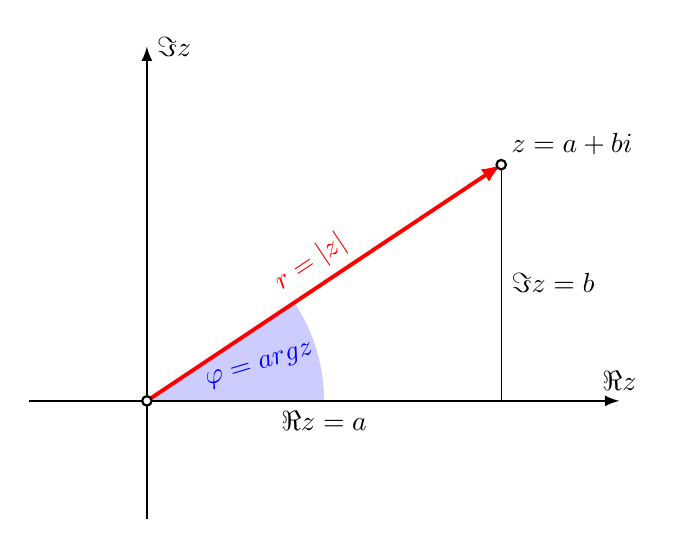
\begin{tikzpicture}[>=latex,thick,scale=1.5]
\pgfmathparse{atan(2/3)}
\xdef\winkel{\pgfmathresult}
\fill[color=blue!20] (0,0) -- (1.5,0) arc (0:\winkel:1.5) -- cycle;
\draw[->] (-1,0) -- (4,0) coordinate[label={$\Re z$}];
\draw[->] (0,-1) -- (0,3) coordinate[label={right:$\Im z$}];
\draw[line width=0.5pt] (3,0) -- (3,2);
\node at (3,1) [right] {$\Im z=b$};
\node at (1.5,0) [below] {$\Re z=a$};
\draw[->,color=red,line width=1.4pt] (0,0) -- (3,2);
\node at (3,2) [above right] {$z=a+bi$};
\def\punkt#1{
	\fill[color=white] #1 circle[radius=0.04];
	\draw #1 circle[radius=0.04];
}
\punkt{(0,0)}
\punkt{(3,2)}
\node[color=red] at (1.5,1) [rotate=\winkel,above] {$r=|z|$};
\node[color=blue] at ({\winkel/2}:1.0)
	[rotate={\winkel/2}] {$\varphi=\operatorname{arg}z$};
\end{tikzpicture}
\caption{Argument und Betrag einer komplexen Zahl $z=a+ib$ in der 
Gaussschen Zahlenebene
\label{buch:zahlen:cfig}}
\end{figure}
Die Zahlenebene führt auf eine weitere Parametrisierung einer
komplexen Zahl.
Ein Punkt $z$ der Ebene kann in Polarkoordinaten auch durch den Betrag
und den Winkel zwischen der reellen Achse und dem Radiusvektor zum Punkt
beschrieben werden.


\subsubsection{Geometrische Interpretation der Rechenoperationen}
Die Addition kompelxer Zahlen wurde bereits als Vektoraddition
in der Gausschen Zahlenebene. 
Die Multiplikation ist etwas komplizierter, wir berechnen Betrag
und Argument von $zw$ separat.
Für den Betrag erhalten wir
\begin{align*}
|zw|^2
&=
z\overline{z}w\overline{w}
=
|z|^2|w|^2
\end{align*}
Der Betrag des Produktes ist also das Produkt der Beträge.

Für das Argument verwenden wir, dass
\[
\tan\operatorname{arg}z
=
\frac{\Im z}{\Re z}
=
\frac{b}{a}
\qquad\Rightarrow\qquad
b=a\tan\operatorname{arg}z
\]
und analog für $w$.
Bei der Berechnung des Produktes behandeln wir nur den Fall $a\ne 0$ 
und $c\ne 0$, was uns ermöglicht, den Bruch durch $ac$ zu kürzen:
\begin{align*}
\tan\arg wz
&=
\frac{\Im wz}{\Re wz}
=
\frac{ad+bc}{ac-bd}
=
\frac{\frac{d}{c} + \frac{b}{a}}{1-\frac{b}{a}\frac{d}{c}}
=
\frac{
\tan\operatorname{arg}z+\tan\operatorname{arg}w
}{
1+
\tan\operatorname{arg}z\cdot\tan\operatorname{arg}w
}
=
\tan\bigl(
\operatorname{arg}z+\operatorname{arg}w
\bigr).
\end{align*}
Im letzten Schritt haben wir die Additionsformel für den Tangens verwendet.
Daraus liest man ab, dass das Argument eines Produkts die Summe der
Argumente ist.
Die Multiplikation mit einer festen komplexen Zahl führt also mit der ganzen
komplexen Ebene eine Drehstreckung durch.
Auf diese geometrische Beschreibung der Multiplikation werden wir zurückkommen,
wenn wir die komplexen Zahlen als Matrizen beschreiben wollen.




